\documentclass[]{article}
\usepackage{graphicx}

%opening
\title{Assignment 5}
\author{Deepak Rishi}

\begin{document}

\maketitle

Q1)

a)

Testing Accuracy of softmax regression (MNIST for ML beginners) is $91.18 \%$.
Training  Accuracy of softmax regression (MNIST for ML beginners) is $91.545 \%$.
\bigskip

Testing Accuracy of Convolutional Neural Network (Deep MNIST for experts) (after running for 1000 iterations and the testing batch size was 1000 in order to fit into the memory.then the mean accuarcy was taken) : $96.23\%$

\bigskip

Training Accuracy of Convolutional Neural Network (Deep MNIST for experts) (after running for 1000 iterations and the training batch size was 1000 in order to fit into the memory, then the mean accuarcy was taken) : $96.334547\%$

\bigskip

Testing Accuracy of the fully connected hidden layer is $86.3\%$ after running for 1000 iterations.

Training Accuracy of the fully connected hidden layer is $86.05\%$ after running for 1000 iterations.


Among all models Convolutional performed the best because it  first learnt the features  and applied max pooling to get translation invariant features as input to the fully connected layer.
This way a very rich set of feature vectors reached the final fully connected layer for classification.

\bigskip

The softmax performed better than the fully connected feed forward because we ran the feed forward neural network for less number of iterations, so the weights of the network for not properly tuned. ON running it for 5000 iterations it out performed SOftmax regression.

\bigskip

b)
\bigskip


Using Rectified Linear Units 

Testing Accuracy of Convolutional Neural Network (Deep MNIST for experts) (after running for 1000 iterations and the testing batch size was 1000 in order to fit into the memory.then the mean accuarcy was taken) : $96.23\%$

\bigskip

Training Accuracy of Convolutional Neural Network (Deep MNIST for experts) (after running for 1000 iterations and the training batch size was 1000 in order to fit into the memory, then the mean accuarcy was taken) : $96.334547\%$

\bigskip

When using Sigmoid Units.


Testing Accuracy of Convolutional Neural Network (Deep MNIST for experts) (after running for 1000 iterations and the testing batch size was 1000 in order to fit into the memory.then the mean accuarcy was taken) : $73.03\%$

\bigskip

Training Accuracy of Convolutional Neural Network (Deep MNIST for experts) (after running for 1000 iterations and the training batch size was 1000 in order to fit into the memory, then the mean accuarcy was taken) : $72.99\%$

\bigskip

Rectified Linear Units outperformed Sigmoid units by approximately $23\%$.
This is because sigmoid units suffer with the problem of Gradient Vanishing and Gradient Explosion (since their derivative is less than 1), i.e. the weights tend to be either very small or very big, thus leading to underfitting or overfitting.

\bigskip
Testing Accuracy of the fully connected hidden layer is $86.78\%$ after running for 1000 iterations.

Training Accuracy of the fully connected hidden layer is $85.95\%$ after running for 1000 iterations.
Rectified Linear units on the other hand do not suffer with that problem since they have a gradient of 1. Thus they lead to better tuning of weights of a  neural network.

\bigskip

c)
\bigskip

Dropout is controlled by $keep-prob$ parameter in Tensorflow.

mean training accuracy with $keep -prob$= 0.25  is   0.951727
the mean test accuracy with $keep -prob$=  0.25  is  0.9535 

\bigskip

mean training accuracy with $keep- prob$= 0.5  is   0.970236
the mean test accuracy with $keep- prob$=  0.5  is  0.9715 

\bigskip

mean training accuracy with $keep- prob$= 0.75  is   0.980691
the mean test accuracy with $keep- prob$=  0.75  is  0.9804
Testing Accuracy of the fully connected hidden layer is $86.78\%$ after running for 1000 iterations.

Training Accuracy of the fully connected hidden layer is $85.95\%$ after running for 1000 iterations.
\bigskip


mean training accuracy with $keep - prob$= 1.0  is   0.987236
the mean test accuracy with $keep-prob$=  1.0  is  0.9831 

\bigskip


As $keep- prob$ is increased from 0.25 to 1 , the overall performance of the Convolutional Network becomes better , when there is a 75\% chance of dropout ($keep-prob=0.25$), most neuron activations will be zero. Hence, most of the neurons will not end up learning anything. Therefore the accuracy is less.

As the keep Probability is increased more neurons get active and learn different representations. Hence, the accuracy increases.

However , no dropout($keep-prob=1$) can lead to overfitting in some cases. Over here it did not. Although, there was not much of an increase in the accuracy as $keep-prob$ increased from $0.75$ to $1$.

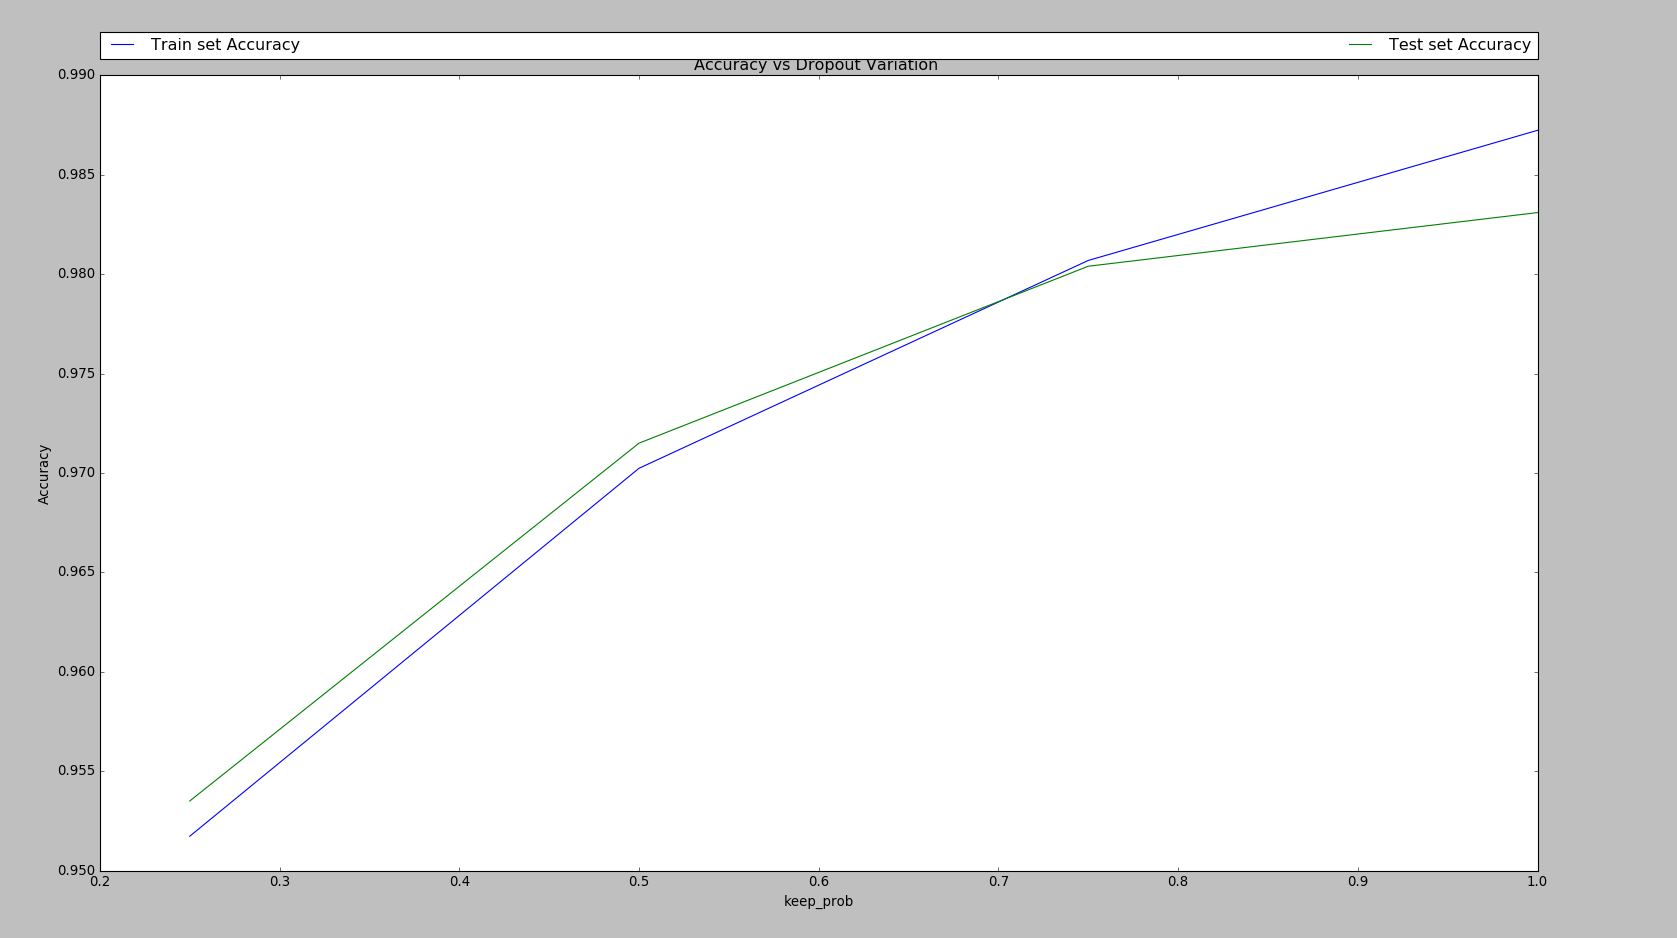
\includegraphics[scale=0.25]{plt.png}


d)

All networks are trained with 1000 iterations.

Fully connected network with  Hidden Layer (150 neurons)

Train set Accuracy= $87.04\%$
Test Set Accuracy= $87.63\%$

Fully connected network with 2  Hidden Layers (128,32 neurons)

Testing Accuracy  is $86.3\%$ 

Training Accuracy  is $86.05\%$ 

Fully connected network with 3  Hidden Layers (85,40,25 neurons)

\bigskip

Testing Accuracy  is $85.13\%$ 

Training Accuracy  is $84.3\%$ 

The best performance was achieved by 1 Hidden Layer of 150 neurons. This is because only 1 layer requires less number of iterations to learn a good set of weights.
Increasing the number of hidden layers led to reduction in accuracy because they were not being trained long enough. The deeper the network , the more backpropogation steps it would require to find the best set of weights.

On increasing the number of iterations the deeper networks perform better.

\bigskip
\bigskip
\bigskip

Q2)

a) This neural network is not  invariant to translations of at most 10 pixels in some direction. This is because it has no max pooling layer.

Consider a situation in which we had a network in which all main objects in the pictures were centered.
The Convolutional Filters will end up learning a set of filters which are dependent on the location of the main objects. Since Convolutional Filters learn a set of $Gabor$ filters initially, there would adapt to the centered image location. After the second set of Convolutional layers, they would not be able to distinguish the image properly if it had been translated.
As the layers progressed the main information of the translated object would be lost since no neoron would be activated correctly by it.


b)

Here the neural network is   invariant to translations of at most 10 pixels in some direction. This is because it has a max pooling layer.

Given one row of an  image  of 30 pixels. The max pooling layer would sample 8 different values from the image. After translating the image by 10 pixels, only the 2 or 3 values in the previous max pooled layer (the non translated image) would change. We would still have 6 (or 5) values from max pooled layer of  the non translated image. Hence this way we preserve most of the content of the translated image from the non translated version.

\end{document}
